\chapter{}{{Data Sets}}{Data Sets}

This chapter describes the three data sets used in the experiments in this thesis. Table \ref{table:data_stats} shows the summary statistics for all three data sets.

\subchapter{Animals with Attributes-2 (AWA2)}
The Animals with Attributes (AWA) data set was originally introduced by Lampert et al.~\cite{DAP}. Since the original images from AWA were not publicly available, Xian et al.~\cite{gbu} enhanced the AWA data set and termed it as Animals with Attributes-2 (AWA2)~\cite{awa}, while retaining the same animal classes and attributes as AWA. AWA2 has a total of 37,322 images compared to 30,475 images in AWA. AWA2 is considered a coarse-grained data set that is medium-scale in terms of images and small-scale in terms of number of classes, i.e. 50 animal classes. The data also provides 85 numeric attribute values for each class. Using the shared attributes, it is possible to transfer information between different classes. The AWA2 data set permits evaluation of the proposed approach in a coarse-grained domain with a small number of classes. A few examples of animal classes in AWA2 are \textit{polar bear}, \textit{zebra}, \textit{otter}, and \textit{tiger}. Figure \ref{image:awa2} shows a few images from the AWA2 data set where the image data was collected from public sources, such as Flickr in 2016. Further information about the data set can be found here \footnote{https://cvml.ist.ac.at/AwA2/}.

\begin{figure}[ht]
\centering
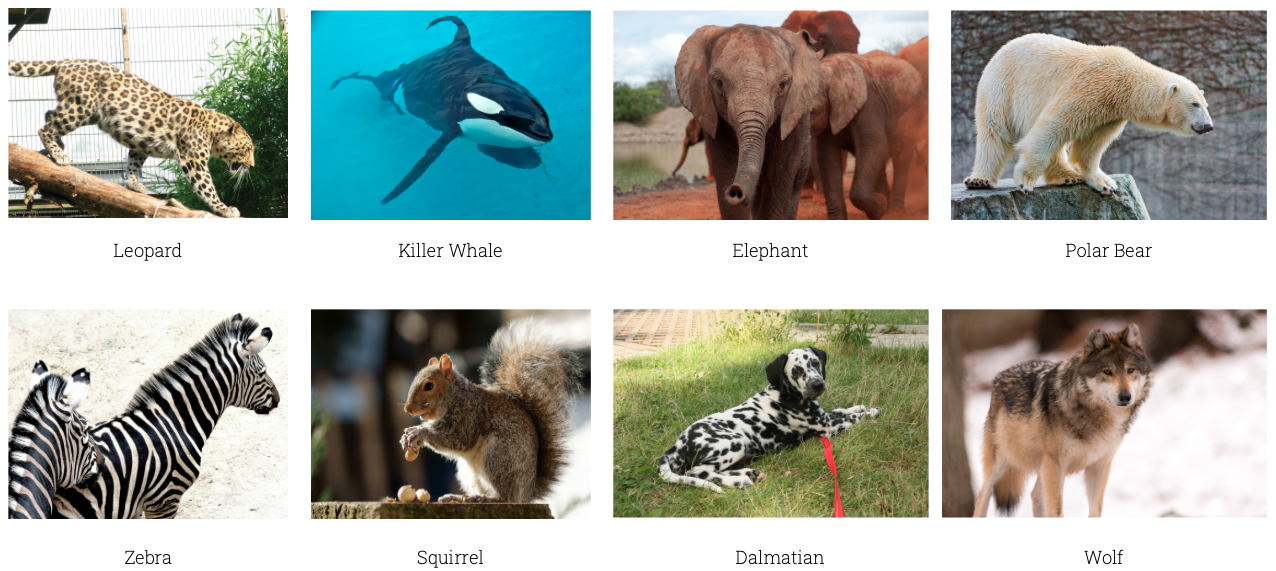
\includegraphics[width=\textwidth]{MS-Thesis-master/figures/awa2_new.png}
\caption{A few labelled images from the Animals with Attributes-2 (AWA2) data set.}
\label{image:awa2}
\end{figure}

\subchapter{Caltech-UCSD Birds (CUB)}

The Caltech-UCSD Birds-200-2011 (CUB) data set~\cite{cub} is an image data set with 11,788 photographs of 200 bird species. Each species is associated with a Wikipedia article and organized by its scientific classification, i.e., (order, family, genus, species). The list of species names was obtained using an online field guide. Each image is annotated with a bounding box, part location, and attribute labels, thereby providing 312 numeric attribute values for each class. CUB is considered a fine-grained data set that is medium-scale in terms of both images and classes. This data set allows evaluation of the proposed approach in a fine-grained domain with a moderate number of classes. A few examples of bird species are \textit{Long tailed Jaeger}, \textit{Blue-winged Warbler}, \textit{American Crow}, \textit{Louisiana Waterthrush}, and \textit{Herring Gull}. Figure~\ref{image:cub} shows a few images from the CUB data set where the images were collected using Flickr image search and then filtered by showing each image to multiple users. Further information about the data set can be found here \footnote{http://www.vision.caltech.edu/visipedia/CUB-200-2011.html}.

\begin{figure}[ht]
\centering
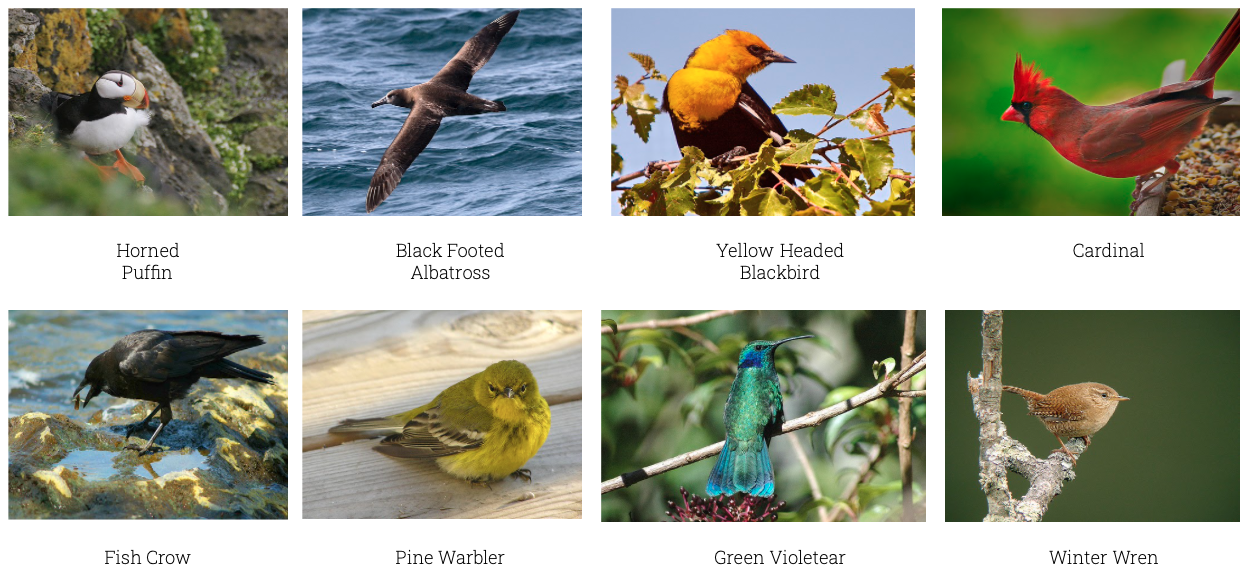
\includegraphics[width=\textwidth]{MS-Thesis-master/figures/cub_new.png}
\caption{A few labelled images from the Caltech-UCSD Birds (CUB) data set.}
\label{image:cub}
\end{figure}

\subchapter{Scene Understanding with Attributes Database (SUN)}
The Scene Understanding with Attributes database (SUN)~\cite{sun} is the first large-scale scene attributes database. A crowd-sourced human study was used to establish a taxonomy of 102 discriminating attributes and the SUN attributes database was built on top of the fine-grained SUN categorical database. The SUN attributes database covers 717 categories and has 14,340 images. SUN is considered a fine-grained data set that is of medium scale in terms of number of images but large scale in terms of number of classes. This data set allows evaluation of the proposed approach in a fine-grained domain with a large number of classes. Few examples of scene classes in SUN are \textit{street}, \textit{indoor brewery}, \textit{valley}, \textit{classroom}, and \textit{supermarket}. The SUN data set also provides a two-level hierarchy for each of the 717 categories. The first level classifies scenes into broad categories such as \textit{indoor}, \textit{outdoor-natural}, and \textit{outdoor-man-made}. The second level further classifies each of the first-level scenes into finer categories such as \textit{workplace}, \textit{shopping}, \textit{forest}, \textit{sports}, \textit{cultural} etc. Figure \ref{image:sun} shows a few images from the SUN data set. The SUN data set is publicly available and further information about the data set can be found here 
\footnote{http://cs.brown.edu/~gmpatter/sunattributes.html}.

\bigskip
\bigskip

\begin{figure}[ht]
\centering
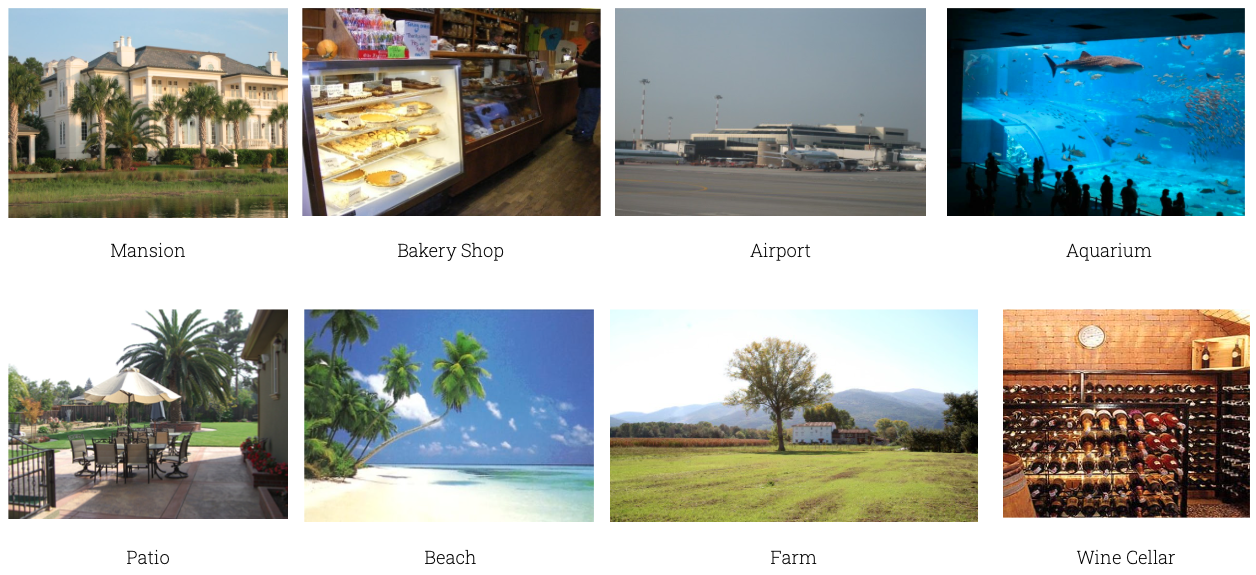
\includegraphics[width=\textwidth]{MS-Thesis-master/figures/sun_new.png}
\caption{A few labelled images from the Scene Understanding with Attributes (SUN) data set.}
\label{image:sun}
\end{figure}


\bigskip
\bigskip

\begin{table}[h]
\centering
\caption{Summary Statistics for all three Data Sets}
\begin{tabular}{@{}lllll@{}}
\toprule
\textbf{Data set} & \textbf{Detail} & \textbf{Classes} & \textbf{Images} & \textbf{Attributes} \\ \midrule
AWA2             & coarse          & 50               & 37,322          & 85\\
CUB              & fine            & 200              & 11,788          & 312\\
SUN              & fine            & 717              & 14,340          & 102\\ \bottomrule
\end{tabular}
\label{table:data_stats}
\end{table}